% ----------------------------------------------------------------------------
%                                 Related Work
% ----------------------------------------------------------------------------
\newpage                                                \chapter{Related Work}

The following section aims to organize previous research enumerating aspects
of both binaural audio and intelligent agents. By exploring prior work in this
space, we begin to observe the benefits arising from the interplay of these
components which will be explored in future work.

%-----------------------------------------------------------------------------%
%                                   Audio
% 1) audio is THE primary element of interface     ~\cite{arons1991hyperspeech}
% 2) audio used to assist user's comprehension         ~\cite{se19993dAudio}
% 3) binaural audio used for HTML presentation         ~\cite{goose19993dAudio}
% 4) binaural audio + other modals     ~\cite{yu2006novel, marentakis2004study}


%-----------------------------------------------------------------------------%
\section{                  Audio Only Interfaces                             }
% 1) audio is THE primary element of interface     ~\cite{arons1991hyperspeech}

MIT's Media Lab has explored the area of "hyperspeech", a corollary to
hypertext where the paradigm is presenting speech as data.  The goal of the
work was to understand the nuances necessary to both extract information from
audio while also accessing it through speech~\cite{arons1991hyperspeech}.

Though speech is an incredible tool for communication, its temporal existence
prevents humans from browsing sounds the way eye can scan text.  Speech and
audio interfaces must be sequential, while visual interfaces can be
simultaneous in nature.  Therefore, designing an interface focused solely on
sound and speech, rather than text, video, or graphics presents a number of
nuanced challenges.  Navigation with speech is much more difficult as
instructions are inherently fleeting, and as Arons demonstrated "one cannot simply
'click here' in the audio domain, for as the selection is made, time has passed
and here has  disappeared"~\cite{arons1991hyperspeech}.

To introduce hyperspeech, or the use of sound as data, Arons conducted interviews
with a number of leading interface design specialists.  The interviews were
brief in nature, completed in approximately 5 minutes.  The speech recorded
from the interview was then processed off line and put into a data base.
Labels and connections were created between associated statements, creating a
graph of the topics discussed.  What was studied was the interface with which
hyperspeech could be used.  The goal of the interface was to answer questions
such as, "How do persons A and B feel about C?" or "Who disagrees with person
A's stance on B?".  Navigation between different topics or through specific
interfaces were studied.

By exploring how the design can influence a user's ability to navigate through
the information of a database, it was demonstrated that it is important to
be able to navigate in any direction arbitrarily from any node. Having all of
the commands available while navigating was the most natural presentation of
an interface.  One benefit of using speech as an input modality is that it is
goal directed and very succinct.  Complexity and variability proved to be a
difficulty when creating this interface.

%%-----------------------------------------------------------------------------%
\section{                 Assistive Audio Interfaces                           }
% 2) audio used to assist user's comprehension      ~\cite{jeon2012listen2droom}

Work by researchers at Georgia Tech demonstrated the use of a single, radial axis 
in an audio interface to present information to blind individuals. They presented
multiple user studies and work of assisting blind users navigate new or unfamiliar
rooms.  With smart phones and computer vision techniques the researchers in 
Bruce Walker's Sonification lab created an application helping blind users understand 
the orientation and placement of objects in new environments. Of note are the 
current practices that blind users employ to navigate these settings. The focus group
Jeon et al. interviewed demonstrated that blind users employ 
various strategies to place objects in a room such as one subjects summarization 
that by "listening to the room, we can detect where running refrigerators, 
computers, or other machinery exists" ~\cite{jeon2012listen2droom}. The second 
most common response was that layout is also often inferred by touch, or assisted
navigation either with the use of inanimate objects (such as walking canes) 
or sighted volunteers. 

The smart phone application presented in this work allows visually handicapped 
individuals to scan a room by holding an external camera connected to the phone, 
or a phone's native camera left to right across the room. The application then
provides the user with 3 modes of information retrieval after video processing 
has been performed to identify the objects and their locations in the environment.

1) Linear Searching : allows the interface to communicate which objects are
present in a room and the order in which they were observed.  The authors found
that this mode allowed users to quickly "scan" a setting and identify whether an 
object of interest existed in the space. 

2) Directional Retrieval: provides the users of the interface with information 
on objects by grouping related objects and returning their location with respect
to room walls and room center.

3) Spatially, using 3D audio, the app vocalizes the position of an object through
the use of binaural audio when the user is wearing a headset. This allows the user
to understand where objects are in relation to their current orientation.

Additionally, the lab has explored optimizations for auditory interfaces. The 
lab demonstrated how the use of spearcons (injections of compressed speech ~\cite{
jeon2009enhanced} that allows the sound to act as a cue within a given context)
can be used to enhance menu navigation on mobile devices ~\cite{
walker2009spearcon}. This work extends previous findings that auditory menus 
that rely solely on TTS vocalizations of the text prove to be much less efficient
than menus that employ spearcons which allow the user to navigate based on injections
and rely on the full speech for context.  This work demonstrates how new constructs 
for navigation can be learned by users, and then used to optimize the navigation
of auditory menus.  Using a Nokia phone with 50 contacts with randomized names,
Walker et al. studied how 89 undergraduates navigated to a target user using 
the visual display only, visual display with TTS, visual display with spearcon,
visuals off with TTS, and then TTS with spearcons. The results show that conditions
with visual cues led to the fastest responses.  Once visuals are disabled, spearcons
helped drive performance to the lower limits, while TTS solution initially afforded
faster initial performance.  With the same amount of practice, spearcons outperformed
TTS engines due to their compressed nature.  This work demonstrates some of the
possible optimizations that can be built in to auditory interfaces.

%-----------------------------------------------------------------------------%
\section{                  Binaural Interfaces                                }
% 3) binaural audio used for HTML presentation         ~\cite{goose19993dAudio}

Researchers at Siemens Corporate Labs demonstrated the comprehensive benefits
of delivering HTML content to users with a binaural interface.  They created
an interactive browser using audio as the primary interface which placed page
elements around a user, focusing on aiding the user maintain orientation while
browsing on the web~\cite{goose19993dAudio}.

The work by Goose et al. was the fist work demonstrating that binaural techniques
could be applied to non prerecorded media. The authors began by researching
how well multiple users could spatialize sound presented to them from regular
PC audio hardware to determine the best design choice for the interface. The
observation that most impacted their design was the inability of most users
to accurately identify the source of sound along the y-axis.  This motivated
Goose et al. to adopt a horizontal axis interface depicted in ~\ref{fig:goose_horizon}.

\begin{figure}[t]
    \centering
    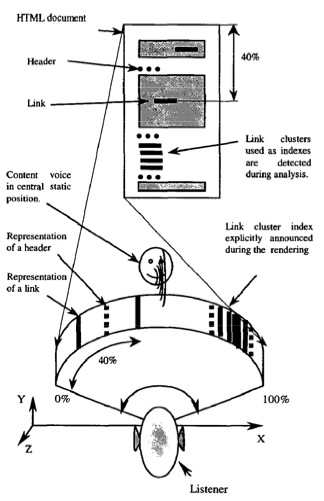
\includegraphics[width=.4\linewidth]{images/goose_horizon.jpg}
    \caption{Mapping an HTML document horizontally}
    \label{fig:goose_horizon}
\end{figure}


By showing the inefficiency of the y-axis to convey accurate information in the
audio space, they demonstrated why an interface simulating the reading down of
a page would be ineffective. Instead, by projecting a document onto the x-axis,
Goose et al. effectively translated web pages into time lines.  The interface
could then compute the length of a given web page by calculating the time it
would take to read.

The horizontal time domain allows the interface to communicate both inter-document
and intra-document links effectively.  To disambiguate the two forms of links,
a "rhetoric of arrival and departure" was created where the interface would
"take-off", "fly", and then "land" in the appropriate section of the horizontal
display as depicted in figure ~\ref{fig:goose_intra}. This rhetoric utilized
unique and specific sounds that the user could associate with given transitions.
With these unique transitions, later tests demonstrated that users could
correctly identify the action performed by links, as well as maintain their
orientation while navigating web pages every time.  Secondly, the interface
could exaggerate this rhetoric by playing the sound of a launch into space,
and then a subsequent landing at the beginning of a new document to
communicate inter-document transitions. This demonstrated the elasticity of
the metaphor which was able to deliver appropriate locational feedback
(similar to scroll bar's location indicating where you are on a page).

Goose et al. also demonstrated how a system can be engineered to prevent a
user from listening to every single document to extract relevant information.
The interface they built allowed for multiple rendering modes (one reads the
document, one that only announced links within a document,  one announcing
section headers).  By having multiple rendering engines, multiple voices
could present different bits of information simultaneously to the user,
allowing the user to focus on the elements of interest when arriving at a
given page.

\begin{figure}[t]
    \centering
    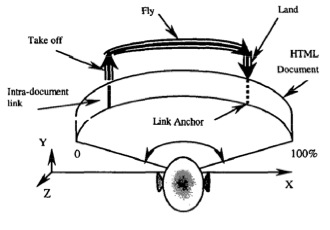
\includegraphics[width=.7\linewidth]{images/goose_intra.jpg}
    \caption{Binaural intra document traversal}
    \label{fig:goose_intra}
\end{figure}

Goose et al provided early results which indicated that binaural audio
improved the user's comprehension of the HTML document's structure and their
overall orientation within multiple pages.  The authors argue that these
factors can improve the effectiveness of the browsing experience for its
users~\cite{goose19993dAudio}.


%-----------------------------------------------------------------------------%
\section{                  Binaural Audio Interfaces with other Modals        }
% 4) binaural audio + other modals     ~\cite{yu2006novel, marentakis2004study}

The viability of this work is exciting when considering how binaural audio
can be used in conjunction with other interfaces.  Research from the
University of Glasgow noted the ergonomics and usability of different tactile
interfaces when coupled with a 3D audio soundscape.  Their work demonstrated
how several interaction patterns (from gestural on mobile devices, to physical
motions such as head nodding) might work with a given soundscape measuring the
tactile interfaces accuracy and effectiveness.  The researchers demonstrated 
some of the difficulties encountered when working with audio as an interface,
citing the ambiguity of 'exact locations' in space when asking subjects to 
locate a sound.  They observed that some of these ambiguities arose from blur
introduced by non-calibrated HRTFs.  Of note are the design choices Marentakis
et al. made when integrating sound and visual displays that allowed for feedback
to the user when guiding the user to interact with a specific sound source.  
They concluded that a 3D soundscape
was effective with all of the tested interfaces and could be used as for
flexible, eyes free interaction with a computer\cite{marentakis2004study}.



%-----------------------------------------------------------------------------%
%                                   Notifications
% notification reliability --> users to ignore  ~\cite{leetiernan2001effective}
% notifications : informative                              ~\cite{maltz2000cue}
% notifications : interpretted                    ~\cite{horvitz1999principles}
% notification systems' users                   ~\cite{cutrell2001notification}
%-----------------------------------------------------------------------------%

%----------------------------------------------------------------------------%
\section{                 HCI : Interface Design                             }

Interface designers focus on three main questions:

\textit{Who is the target user?}

\textit{What is the task the user is trying to accomplish?}

\textit{How can you make an interface that is the most sensible for this task?}

These design principles were established to make computers more usable and
receptive to a user's immediate needs. The goal of designing the best interface
with given constraints, simultaneously optimizing for a desired property (such
as efficiency or learn-ability) is not a trivial undertaking.

The field of HCI as such, experiments with new design methodologies and
hardware, prototyping new systems, and exploring new paradigms for interaction
to minimize the  barriers between the human's cognitive model of what they are
trying to accomplish and the computer's representation of the task
~\cite{baecker1987human}. The following sections explore findings of each goal
as presented in the current research.  What is important to note is that this
project, though geared towards users with visual disabilities, adheres to
the mantra of maximizing human cognitive and physical abilities using the
guidelines found in~\cite{reeves2004guidelines}.

\section{                  Psychology of Interface Design                    }

The interplay of ergonomics and psychology are known facets of HCI. As such, 
the design of novel interfaces are encouraged to either increase efficiency or 
user satisfaction (preferably both). To more concretely enumerate the goals, 
the literature provides a number of guiding examples.  Exploring a number of 
different goal oriented tasks, general patterns of interactions emerge that 
suggest a conversational metaphor would be an appropriate interface design 
choice because the user could leverage existing biological mechanisms to 
understand the interface and that the existing conversational mental model 
directly supports direct and simple inference of what information this 
interface is presenting~\cite{kieras1984role}.

\subsection{                  Mental Models and Cognitive Loads              }

A limitation of most interfaces is simply the size and volatility of a user's
short term memory.  To make real time captioning easier for untrained works
Lasecki et al. demonstrated how time could be warped for any given users task.
Warping the playback speed of previously recorded audio enabled users to perform
the captioning task more efficiently by reducing the high cognitive load needed 
for captioning ~\cite{lasecki2013warping}.

Simplifying information is not only beneficial for goal oriented and task driven
processes, but they are also empirically preferred by users of a number of
systems. Exploring a users collective preference for simpler  representations of
information, Patel et al. demonstrated that users preferred summarized
directions that incorporated familiar paths to more detailed and exact routing
instructions. The users in the study valued traveling on  familiar routes enough
to sacrifice overall trip distance and travel time
required~\cite{patel2006personalizing}.

When an interface is controlled by a semi-autonomous intelligent agent, it
becomes increasingly important to be aware of the interactions that users will
have with the system as decisions are being made.  In this system, the
decisions that would be made relate to the verbosity for a given notification,
the position to place the notification relative to the user, and what actions
are available to the user when acting on a notification.  Prior work has
explored how an intelligent agent can explain itself to the user, the amount
varying degrees by which an intelligent agent can reconfigure itself, and the
effects of a user's mental model soundness~\cite{kulesza2012tell}.

\subsection{                   Mental Model Elasticity                       }

Since Irys is an exploration of a new interaction technique, it's important to
consider user's ability to learn how the system works. Work in HCI explores how
well users are at creating new mental models for interactions as evidenced by
shifting paradigms of technology hardware (changing from numeric keypads, to
stylus, to keyboard, to touchscreen).  Work from the Universitite Paris Sud
explored how well users could remap existing mental models by exploring how
users adapt to interaction techniques that use the temporal dimension versus
more advanced uses of rhythmic patterns to convey information.  The researchers
explored how rhythmic techniques, though a deviation from  user expectation of
temporal interactions (such as multiple clicks), can be particularly useful in
situations where the visual channel is overloaded or even not available.  They
concluded that  (i) rhythmic patterns can be efficiently reproduced by novice
users and recognized by computer algorithms, and (ii) rhythmic patterns can be
memorized as efficiently as traditional shortcuts when associating them with
visual command~\cite{ghomi2012using}.  This work suggests that deviations from
common interaction patterns can be beneficial to users when training is
provided.

\section{                  Interface Elements                                }

Eric Horvitz depicted the divide in research focusing on the promise of creating
new metaphors and tools that enhance a user's ability to directly manipulate
objects \textit{versus} an applications ability to provide automation. In his
system LookOut, Horvitz explored the role of a user interface in guiding the
user to task completion.  He explained the benefits of building an interface
that tailored the computer to drive task completions through what he coined as
"Mixed Initiative" actions.  He demonstrated how different modalities of
interactions could allow a system to overcome uncertainty while delighting the
user with a perceived automated experience that performed repetitive tasks for
the user~\cite{horvitz1999principles}.  This application demonstrated how user
interfaces could adapt to noisy data, such as uncertainty about times referring
to an event that needs to be scheduled in an email. The influence LookOut has on
modern interfaces can be seen with many common email clients such as Google's
Gmail and Microsoft's Outlook performing similar mixed-initiative actions.  In
relation to Irys, the system will have to learn how to notify users of changes
by evaluating the costs and benefits associated with interruptions at different
times.

\subsection{                  Visual Notifications                           }

While performing a task, it is important that an interface assists the user to
work efficiently. Certain assumptions are made between the user and the interface
as they are in fact entering a working relationship.  When using an interface,
users inherently trust that the system will assist them in completing tasks.
The question of a users trust in a system is therefore important when designing
notification interfaces, with the goal being mitigating all negative first
impressions.  Empirical evidence shows that users carry a historical bias when
dealing with actionable notifications \cite{leetiernan2001effective}.

The study of information design and the options that are suitable for three often
conflicting design objectives for notifications - interruption to primary tasks,
reactions to specific notifications, and comprehension of information over time
- are necessary to create the most efficient computing environment.
Understanding the impact visual notifications have on a user directly inform the
decisions made for an audible interface.

Given the stochastic nature of notifications, probabilistic reliability can be
used to create intelligent messaging systems that gain a user's trust, rather
than lose it~\cite{leetiernan2001effective}. Empirical evidence show that users
will ignore all notifications that are not highly valid when performing
demanding visual tasks~\cite{maltz2000cue}, but there are also findings that
demonstrate that a notifications timing determines the amount of disruption it
causes a user ~\cite{cutrell2001notification}.  In a study, Microsoft
Researchers found that notifications occurring at the beginning of a task are
more likely to completely derail focus while those occurring near the completion
of tasks have mitigated effects.

\section{                  Tactile Notifications                             }

When exploring non-visual interfaces, it is important to consider how the human
mind operates when interfaces utilize other sensation modalities. Consider
interfaces that utilize haptic feedback.  It has been shown that for many
dynamic tasks (such as remote control of robots), haptic interfaces are able to
provide the user with important types of feedback.  For example, a user is able
to detect the same forces that might impede the operation of the target object.
In other situations, users may prefer haptic feedback to audible interactions
when in social situations where audible interruptions are discouraged.  Other
uses of haptic interfaces are seen in high precision tasks (such as surgery)
where it is important to apply the precise torques and forces on both ends.
Common to all of these interfaces is the purpose of the device is human
actuation, often at a physically smaller interface~\cite{ellis1996design}.
There has been work looking at the psychophysical use of power amplification
as seen in prosthetic engineering, but those are not considered for this
project.

What is of note is that interfaces that utilize haptic feedback are often set in
a master/slave relationship between the user and the object on the other end of
the interface. Complexity is often measured in degrees of freedom that the
operator has over the slave device.  What is important with haptic feedback is
that notifications have to be performed in real-time or else stale information
propagates into large control errors~\cite{ellis1996design}.

\section{                  Auditory Notifications                            }

SOCIAL ISSUES: In their paper Hanson et al. discussed the interplay of social
situations and auditory cues~\cite{hansson2001subtle} Current auditory
notifications cues can be attention demanding, distinct, and can be perceived as
intrusive in social situations. "The beeping and ringing is by nature an
intrusive sound not unlike the sound of an alarm clock" referring auditory cues
often heard arising from cell phones  ~\cite{hansson2001subtle}.  Nitin Sawhney
performed an empirical study demonstrating how existing devices with audible
notifications (read: pagers and phones) can detract from an owner's
concentration throughout a day.  Their work demonstrated that there was around
10 minutes per hour spent on  interruption handling by the average user in their study.
To address this issue, researchers at MIT created Nomadic Radio, a physical
device that would infer when the ideal time to present a notification to the
user by listening to the environment~\cite{sawhney1999nomadic}. In this paper,
the researchers provide a mechanism for scaling a cue to the user providing
the user with the ability to prevent an interruption. Other techniques are
presented to allow the user to quickly identify senders based on items such as
auditory signatures.  Of interest is the fact that the ambient auditory
introduction was the most requested feature as user's cited the least cognitive
effort required to anticipate the subject or content of the new notification.
